\documentclass{article}

% Lenguaje y Fuente
\usepackage[spanish]{babel}
\usepackage[utf8x]{inputenc}
\usepackage[T1]{fontenc}
\usepackage[top=1in, bottom=1.25in, left=1.1 in, right=1.1 in]{geometry}
\usepackage{graphicx}
\usepackage{ragged2e}
\usepackage[usenames]{color}
\usepackage{multicol}

% Portada

\title{\textbf{Reporte de la Actividad 9}\\ Solución numérica de ecuaciones diferenciales ordinarias}
\author{Luis Fernando Duarte Gonzalí \\ Universidad de Sonora \\ Física Computacional}
\date{Mayo del 2019}
\begin{document}
\maketitle

% Contenido del Reporte

\section{Introducción}

En esta actividad nos introducimos a Python para resolver numéricamente un sistema de ecuaciones diferenciales ordinarias. Python cuenta con librerías como SciPy y Numpy, las cuales se pueden utilizar para encontrar soluciones numéricas de ecuaciones diferenciales.

En esta actividad, se resolvió numéricamente un sistema de ecuaciones diferenciales ordinarias que describen el sistema que aparece en la siguiente figura. Nos basamos en las notas de Richard Fitzpatrick, de la Universidad de Texas que resuelve analíticamente el sistema mencionado.

\begin{center}
    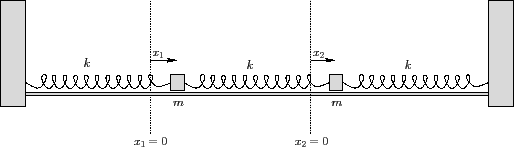
\includegraphics[scale = 0.5]{springs.png}
\end{center}

\section{Teoría}
\subsection{Problema de dos masas acopladas a resortes}

Considera un sistema mecánico que consiste en dos masas idénticas $m$ que son libres para deslizarse sobre una superficie horizontal sin fricción. Supongo que las masas están atadas una a la otra, y a dos paredes inamovibles, refiriendonos a que hay tres resortes ligeros idénticos colocados horizontalmente con constante elástica $k$ como se mostró en la primera figura en la sección de Introducción. El estado instantáneo del sistema está convenientemente especificado por los desplazamientos de la masa de la izquierda y de la derecha, $ x_1(t)$ and $ x_2(t)$ , respectivamente. Las extensiones de los resortes de la izquierda, medio, y derecha son  $ x_1$ , $ x_2-x_1$ , y $ -x_2$, respectivamente, asumiendo que $ x_1=x_2=0$ corresponde a la configuración de equilibrio en donde los resortes están todos en su forma natural. Las ecuaciones de movimiento de las dos masas son:
\begin{equation}
    m \ddot{x}_1 = -k x_1 +k (x_2-x_1)
\end{equation}
\begin{equation}
        m \ddot{x}_2 = -k (x_2-x_1) + k (-x_2)
\end{equation}
En la figura hemos hecho uso del hecho de que una masa atada al final izquierdo de un resorte de extensión $x$ y constante elástica $k$ experimenta una fuerza horizontal $+k x$, en cambio la masa atada al final derecho del mismo resorte experimenta una fuerza igual y opuesta $-kx$.

\subsection{Procedimiento}
Primero nos basamos en el código que aparece en el Cookbook de SciPy, adaptando el problema de las notas de R. Fitzpatrick. Como primer paso, comprendimos los elementos y partes del código de la página del Cookbook de SciPy y lo hicimos correr.

En el que el problema era muy parecido, sólo que faltaba una pared y con ella un resorte atado a la derecha de la segunda masa.
\begin{center}
    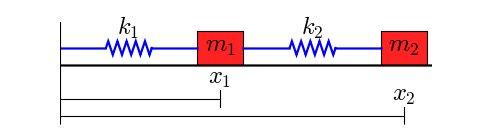
\includegraphics[scale = 0.65]{two_springs_diagram.png}
\end{center}
Y las ecuaciones diferenciales que describen al sistema son las siguientes:
\begin{equation}
    m_1 \ddot{x}_1 + b_1 \dot x_1+k_1 (x_1 − L_1) − k_2 (x_2 −x_1 − L_2) = 0
\end{equation}
\begin{equation}
    m_2 \ddot{x}_2 + b_2 \dot x_2 + k_2 (x_2 − x_1 − L_2) = 0
\end{equation}
Para poder resolver mediante SciPy es necesario hacer una conversión de el sistema anterior a uno de primer orden. Las variables serían:
\begin{equation}
    y_1 = \dot x_1
\end{equation}
\begin{equation}
    y_2 = \dot x_2        
\end{equation}
Las cuales son las velocidades de las masas $m_1$ y $m_2$. Ahora sólo tenemos 4 ecuaciones de primer orden cada una:
\begin{equation}
    \dot x_1 = y_1
\end{equation}
\begin{equation}
    m_1 \dot y_1 + b_1 y_1 + k_1(x_1 - L_1) - k_2 (x_2 - x_1 - L_2) = 0
\end{equation}
\begin{equation}
    \dot x_2 = y_2
\end{equation}
\begin{equation}
    m_2 \dot y_2 + b_2 y_2 + k_2 (x_2 - x_1 - L_2) = 0
\end{equation}

\section{Resultados}
Tomamos como parámetros:
$$m_1=m_2=0.25$$
$$k_1=k_2=k_3=10$$
$$L_1=L_2=1$$
$$b_1=b_2=0$$
Y las condiciones iniciales:
$$x_1 = 2.0$$
$$y_1 = x_2 = y_2 = 1.0$$
\clearpage

La gráfica generada con los parámetros fue la siguiente
\begin{center}
    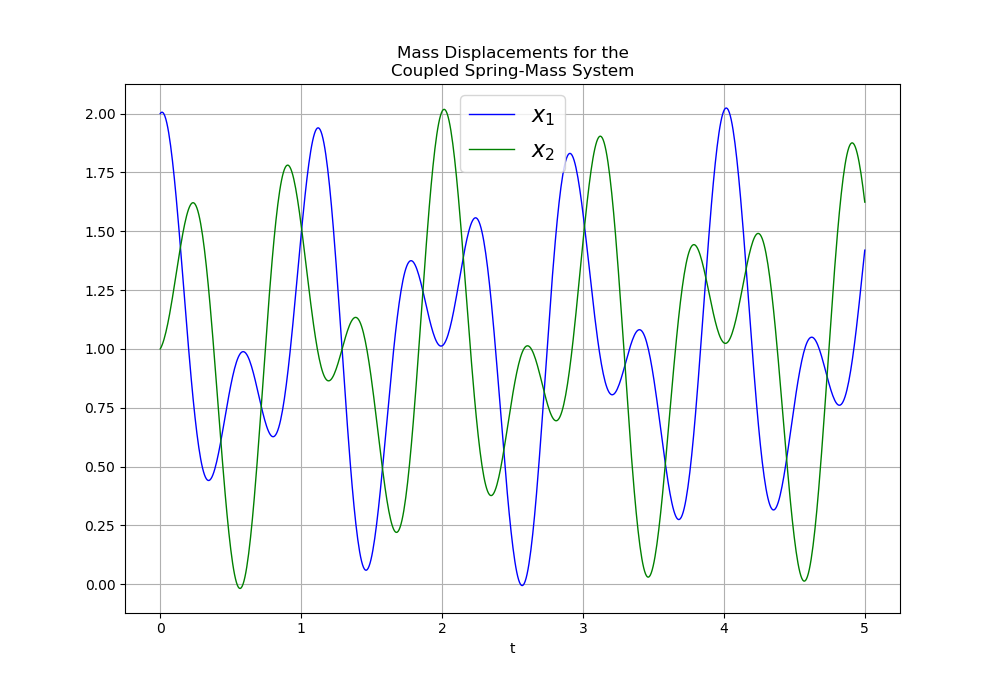
\includegraphics[scale = 0.4]{two_springs.png}
\end{center}
Y se buscaba replicar la siguiente gráfica
\begin{center}
    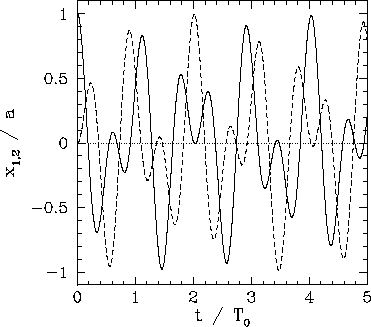
\includegraphics[scale = 0.5]{two_springs_original.png}
\end{center}

\section{Conclusión}
A modo de conclusión podemos decir que Python es un lenguaje bastante flexible que en esta práctica demuestra que se puede usar para resolver ecuaciones diferenciales de manera numérica, además de ser bastante rápido.

\section{Referencias}
\begin{itemize}
    \item Two Spring-Coupled Masses. Sitio web:
    
    https://farside.ph.utexas.edu/teaching/315/Waves/node18.html
    
    \item Función odeint. Consultado de SciPy.org. Sitio web:
    
    https://docs.scipy.org/doc/scipy/reference/generated/scipy.integrate.odeint.html
    
    \item Coupled spring-mass system. Consultado de SciPy Cookbook. Sitio web: 
    
    https://scipy-cookbook.readthedocs.io/items/CoupledSpringMassSystem.html
\end{itemize}
















\end{document}
